% Chapter 1

\chapter{Tips} % Main chapter title

\epigraph{``Y a plein de c\^otes \`a Ibiza\\C'est vraiment dur il fait tr\`es chaud.''}{\textit{Zambla}}

\label{chapter1} % For referencing the chapter elsewhere, use \ref{Chapter1}

%----------------------------------------------------------------------------------------
\section{Introduction}
Dear student reading that chapter, greetings!
After doing some research and writing reports for more than 12 years, I realized that LaTeX is the second worst way to write a thesis.
The worst one is Word.
Then you may be wondering, which is the best way to write a report?
Well, actually there is no best way.
Hence you are stuck with LaTeX.

\subsection{Goal of this chaper}
In this chapter, I will demonstrate a few interesting features of LaTeX, and more importantly, provide examples of Figures, Tables, Equations and Code Snippets.
These may be easy to deal with on Word, but here it is another story.
The general idea is to keep these examples, copy-paste them, then modify them to fit your needs.
If you are seeing this content while reading \texttt{main.pdf}, please load the overall LaTeX project in your LaTeX editor, and open the \texttt{chapters/chaper1.tex}.
\\
\\
Done?
Ok let us move on then!
So by now, you should have noticed a few things:
\begin{itemize}
  \item Each sentence of the text is on a distinct line. Yet, sentences are still within the same paragraph.
  \item Backslash is an escape character, used at the beginning of LaTeX commands.
  \item To end a paragraph (or actually insert a newline), we can use the \textbackslash{}\textbackslash{} command.
\end{itemize}
Also now you know how to do a bullet list.

\subsection{Structure of a chapter}
Chapter contain sections (defined with \textbackslash{}section\{Name of your section\}), subsections (\textbackslash{}subsection).

\subsubsection{Because subsubsection that's why!}
Subsubsections are also available (\textbackslash{}subsubsection).

\paragraph{Paragraph}
If you really insist, there are also paragraphes, which may or may not be the same as a subsubsection.
Note that the automatically generated table of contents only goes to two levels of depth within chapters by default.
This can be changed, but you likely do not want to do that.

\subparagraph{Subparagraph}
I was today years old when I discovered the subparagraph. Seriously, do not use it.

\section{Font Formatting Commands}
Similarly to Word, LaTeX provides simple formatting, including \textbf{bold}, \textit{italic}, \underline{underlined} and \texttt{ugly stuff}.
However, no underline or strikethrough by default.
You can also change the size of the text, using {\tiny tiny}, {\small small}, {\large large}, {\huge huge}.
These last commands work within a specific scope.
The scope can be specified using \{ and \}, with the \{ placed before the \textbackslash{}size command.

\subsection{Special characters}
LaTeX uses 10 special characters. Each of these characters has a special meaning.
\begin{enumerate}
  \item Ampersand (\&) is used in tables as a cell delimiter.
  \item Percent sign (\%) is used for commenting a line.
  \item Dollar sign (\$) is used to switch back/from mathematical notation mode.
  \item Hash sign (\#) is used to create macros --- you definitely do not want to go more in depth here.
  \item Underscore (\_ or \textunderscore) is used to indicate a subscript in maths mode, if you use it in text mode ( without using backslash in front to ''escape'' it), your project will not compile anymore. \textbf{You may want to read that twice, and remember it.} It is in a LaTeX template, therefore it must be true.
  \item Curly brackets (\{ and \}) or bracets are used by LaTeX commands, as you likely already noticed.
  \item Tilde (\textasciitilde) can be used to create a non-breaking space (so that both words are on the same line).
  \item Caret/Circumflex/Hat (\textasciicircum) is used to indicate superscript (exponent) in maths mode.
  \item Backslash (\textbackslash) is used in front of every command. You cannot simply escape it to print it, as \textbackslash{}\textbackslash{} create a new line.
\end{enumerate}
If you happen to insert some of these symbols in your text without either escaping (when possible) or using the correct command, your project will likely not compile.
Thus, you may want to be extra careful about that problem.
Note: the underscore issue may also be encountered with bibliography.
So if \texttt{bibtex} displays an error, it may also come from an underscore somewhere in the abstract, DOI or URL field.

\section{Equations}
Here is an equation:
\begin{equation}
\int_0^\infty e^{-x^2} dx
\label{eq:eq1}
\end{equation}

I could also want to have this equation inline, i.e. within the text: $\int_0^\infty e^{-x^2} dx$.
In that case, simply use \textdollar{} (by the way, note that using the dollar sign in your text switches to mathematical notation. To actually print a dollar sign use the \textbackslash{}textdollar command).
The equation above has a label, meaning you can refer to it. The numbering system uses the chapter number (in this case 1), then the equation position within the chapter (1 again).
Example: Equation~\ref{eq:eq1} is an example of an equation in LaTeX{}.
In case you would like to have an equation without numbering it? Easy!
\begin{equation*}
t = a \times log_{2}(\frac{D}{W} + 1) + b
\end{equation*}

The only difference? The \textasteriskcentered{}  symbol in the \textbackslash{}begin\{equation\textbf{\textasteriskcentered}\}.
This also works with Figures and Tables.

\section{Code Snippets}

\begin{lstlisting}
  int main (int argc, char ** argc)
  {
    printf("Hello world!\n");
    return 0;
  }
\end{lstlisting}

This template uses the \texttt{lstlisting} package, which not the best for code snippets.
However, it works without any problem, while other packages may have compatibility issues.
Feel free to try alternative solutions, the best one being \texttt{minted}.

\section{Figures}
Figures are a bit tricky with LaTeX {\tiny(not as much as tables though)}.
Let us see a simple example below:
\begin{figure}[!h]
  \centering
    
\includegraphics[width=0.9\textwidth]{figures/future.png}
  \caption{When a YNC alumni tells you that back in their days, they did not have LaTeX template and would write their report in latin on a papyrus.}
  \label{fig:future}
\end{figure}
You can refer to it: Figure~\ref{fig:future}.
This is possible thanks to the \textbackslash{}label command.
The figure should also be shown on the \hyperref[lst:figs]{List of Figures} page (note this other way of referring to another part of the manuscript!).
A common practice is use the following naming convention:
\begin{itemize}
  \item A prefix, indicating the nature of the object labelled: \texttt{eq} for equations, \texttt{fig} for figures, \texttt{tab} for tables.
  \item A colon.
  \item A unique name (easy to remember) describing your figure. Example: exp1confmatrix would suggest that the figure shows a confusion matrix for your experiment 1.
\end{itemize}

A few other points: The \textbackslash{}caption and \textbackslash{}label can be put either before or after the \textbackslash{}includegraphics command.
When you create a Figure, you need to provide placement information for LaTeX. LaTeX will usually not locate the figures \emph{exactly} where you want them.
The most common specifiers are: \texttt{h} (here), \texttt{b} (bottom of the page) and \texttt{t} (top). The \texttt{!} specifier tries to force LaTeX to put the image exactly at the location you specified (with mixed success though).
For a longer list of specifiers, please refer to: \url{https://en.wikibooks.org/wiki/LaTeX/Floats,_Figures_and_Captions}.

\subsection{Figure Size}
The size of the figure can be determined by the first parameter of the \textbackslash{}includegraphics command.
In this example, we set the size to be $0.9 \times \texttt{textwidth}$, or 90\% of the size of a column.
We could have used an absolute value in cm, e.g. \texttt{width=19cm}.

\subsection{Supported Formats}
Use standard formats, such as PNG, PDF, JPG.
LaTeX also supports other formats, such as EPS.
\textbf{Rule of thumb: use PDF as much as you can, as it uses vector graphics, making it easy to scale the figure to very large format without problems.}

\subsection{Multiple images in one figure}
You can also create complex figures with multiple images.
Here is an example, which uses a $2\times2$ layout.
The overall figure can be referred as Figure~\ref{fig:drake}.
\begin{figure}[!h]
  \begin{subfigure}[t]{.5\textwidth}
    \centering
    
\includegraphics[width=\linewidth]{figures/draketl.png}
    %\caption{We could totally insert a caption here}
    %\label{fig:draketl}
  \end{subfigure}
  \hfill
  \begin{subfigure}[t]{.5\textwidth}
    \centering
    
\includegraphics[width=\linewidth]{figures/draketr.png}
    %\caption{We could totally insert a caption here}
        %\label{fig:draketr}
  \end{subfigure}

  %\medskip
  % the medskip will have white space between both lines
  \begin{subfigure}[t]{.5\textwidth}
    \centering
    
\includegraphics[width=\linewidth]{figures/drakebl}
    %\caption{We could totally insert a caption here}
        %\label{fig:drakebl}
  \end{subfigure}
  \hfill
  \begin{subfigure}[t]{.5\textwidth}
    \centering
    
\includegraphics[width=\linewidth]{figures/drakebr}
    %\caption{We could totally insert a caption here}
    %\label{fig:drakebr}
  \end{subfigure}
  \caption{Example of a complex figures on a $2\times2$ layout.}
  \label{fig:drake}
\end{figure}

\section{Tables}
Tables can be a nightmare in LaTeX.
The easiest way to deal with tables in LaTeX is to use some online tools.
My favorite so far: \url{https://www.tablesgenerator.com/}

Here is an example of confusion matrix generated:
\begin{table}[!h]
  \resizebox{\textwidth}{!}{
\begin{tabular}{|c|c|ccccccccc}
\cline{1-2}
Chest (C)                         & -     &                                                                          &                                                                           &                                                                          &                          &                            &                           &                           &                            &                                                                            \\ \cline{1-3}
Chest (ND)  & *     & \multicolumn{1}{c|}{-}                                                   &                                                                           &                                                                          &                          &                            &                           &                           &                            &                                                                            \\ \cline{1-4}
Chest (D)   & *     & \multicolumn{1}{c|}{-}                                                   & \multicolumn{1}{c|}{*}                                                    &                                                                          &                          &                            &                           &                           &                            &                                                                            \\ \cline{1-5}
Ear          & -     & \multicolumn{1}{c|}{-}                                                   & \multicolumn{1}{c|}{-}                                                    & \multicolumn{1}{c|}{}                                                    &                          &                            &                           &                           &                            &                                                                            \\ \cline{1-6}
Thigh       & *     & \multicolumn{1}{c|}{-}                                                   & \multicolumn{1}{c|}{*}                                                    & \multicolumn{1}{c|}{*}                                                   & \multicolumn{1}{c|}{-}   &                            &                           &                           &                            &                                                                            \\ \cline{1-7}
Neck        & -     & \multicolumn{1}{c|}{*}                                                   & \multicolumn{1}{c|}{-}                                                    & \multicolumn{1}{c|}{*}                                                   & \multicolumn{1}{c|}{-}   & \multicolumn{1}{c|}{-}     &                           &                           &                            &                                                                            \\ \cline{1-8}
Palm        & -     & \multicolumn{1}{c|}{}                                                    & \multicolumn{1}{c|}{*}                                                    & \multicolumn{1}{c|}{-}                                                   & \multicolumn{1}{c|}{-}   & \multicolumn{1}{c|}{-}     & \multicolumn{1}{c|}{-}    &                           &                            &                                                                            \\ \cline{1-9}
Thumb       & -     & \multicolumn{1}{c|}{*}                                                   & \multicolumn{1}{c|}{-}                                                    & \multicolumn{1}{c|}{*}                                                   & \multicolumn{1}{c|}{-}   & \multicolumn{1}{c|}{-}     & \multicolumn{1}{c|}{*}    & \multicolumn{1}{c|}{*}    &                            &                                                                            \\ \cline{1-10}
Inner Wrist & *     & \multicolumn{1}{c|}{-}                                                   & \multicolumn{1}{c|}{-}                                                    & \multicolumn{1}{c|}{-}                                                   & \multicolumn{1}{c|}{*}   & \multicolumn{1}{c|}{*}     & \multicolumn{1}{c|}{*}    & \multicolumn{1}{c|}{-}    & \multicolumn{1}{c|}{*}     &                                                                            \\ \hline
Outer Wrist & -     & \multicolumn{1}{c|}{*}                                                   & \multicolumn{1}{c|}{-}                                                    & \multicolumn{1}{c|}{*}                                                   & \multicolumn{1}{c|}{-}   & \multicolumn{1}{c|}{-}     & \multicolumn{1}{c|}{-}    & \multicolumn{1}{c|}{*}    & \multicolumn{1}{c|}{-}     & \multicolumn{1}{c|}{-}                                                     \\ \hline
  & Belly & \multicolumn{1}{c|}{\begin{tabular}[c]{@{}c@{}}Chest\\ (C)\end{tabular}} & \multicolumn{1}{c|}{\begin{tabular}[c]{@{}c@{}}Chest\\ (ND)\end{tabular}} & \multicolumn{1}{c|}{\begin{tabular}[c]{@{}c@{}}Chest\\ (D)\end{tabular}} & \multicolumn{1}{c|}{Ear} & \multicolumn{1}{c|}{Thigh} & \multicolumn{1}{c|}{Neck} & \multicolumn{1}{c|}{Palm} & \multicolumn{1}{c|}{Thumb} & \multicolumn{1}{c|}{\begin{tabular}[c]{@{}c@{}}Inner\\ Wrist\end{tabular}} \\ \hline
\end{tabular}
}
\caption{Post-hoc comparisons between body parts. - shows no significant difference ($p>.05$), \textasteriskcentered{} shows differences ($p<.05$).}
\label{tab:posthoc}
\end{table}

Note that a table is actually a container for another type of LaTeX object, \emph{tabular}.
Tables come with captions and label, allowing us to refer to Table~\ref{tab:posthoc}.
Another interesting point is that the \textbackslash{}begin\{tabular\} command uses characters.
These characters specify how the text should be centered within each cell: \texttt{c} means centered, \texttt{l} means left and \texttt{r} means right.
Finally, my original table was too large to fit a page, so I used the \textbackslash{}resizebox\{\textbackslash{}textwidth\}\{!\}\{ command.
This command needs a closing \} after the \textbackslash{}end\{tabular\} command.
This table is also now shown in the \hyperref[lst:tabs]{List of Tables} page.
\\
\textbf{Anyway, for Tables, using the LaTeX Table Generator is a great option.}

\section{Bibliography}
LaTeX{} is really convenient to deal with bibliography.
All your references should be in a \texttt{\textasteriskcentered.bib} file.
Each reference has a unique key, that you will use to refer to that publication.

You can simply cite nearly anything using the \textbackslash{}cite command.
You can cite conference papers, e.g. ``WatchIt (\cite{Perrault2013}) is an interactive wristband for smart watches.'' or journal articles, e.g. ``Lopez et al. (\cite{Lopez2017}) ran a public consultation in Mexico''.
In the first example, the key in the bib file is Perrault2013, see\\

\includegraphics{figures/bibtexkey}

\subsection{How to get Bibtex References?}
The easiest way to find the Bibtex snippet you need for a given reference is to use Google Scholar~(\cite{Scholar}).
On the main page, type the name of the paper you are looking for.
\\

In the results page, locate the paper:
\begin{figure}[!h]
  \centering
    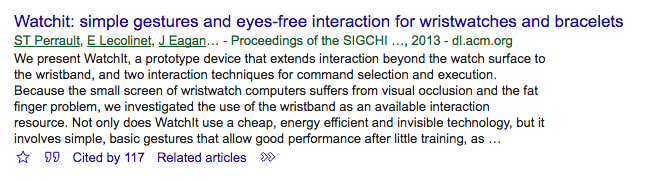
\includegraphics[width=0.9\textwidth]{figures/scholarrefexample.png}
  \caption{Example of result on Scholar}
  \label{fig:scholarref}
\end{figure}

On the last line of the result (shown in Figure~\ref{fig:scholarref}), there is a \textbf{''} symbol.
Clicking on it will display a pop-up.
\begin{figure}[!h]
  \centering
    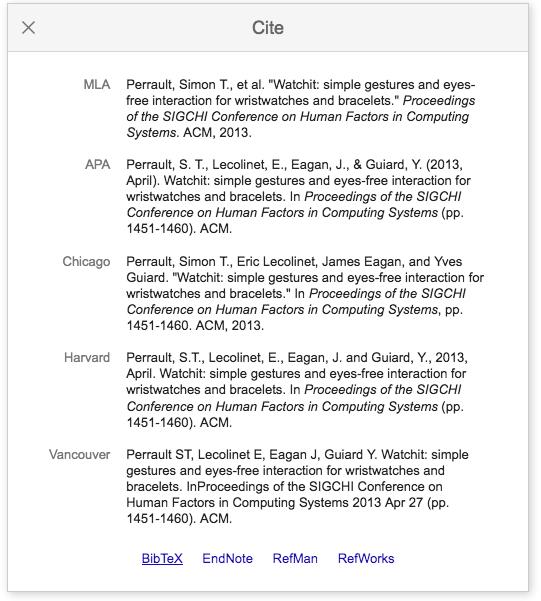
\includegraphics[width=0.7\textwidth]{figures/scholarpopup.png}
  \caption{Pop-up window with the possible citations}
  \label{fig:scholarpopup}
\end{figure}
\\

At the bottom (see Figure~\ref{fig:scholarpopup}), you will notice a ``Bibtex'' link. Click on it.
Scholar will then display a small block of text starting with @ symbol.
Copy and paste this snippet in your \texttt{biblio.bib} and you are done.
You may eventually want to check the citation key to something shorter.
\\

\textbf{You may get unexpected compilation errors with some references. The most common case is that the bibtex entry contains a DOI field, which in turn contains an underscore (\_).}
If that is the case, simply remove the DOI field (not a great practice but a good workaround).

\section{End of the Tips}
We are now done with the tips.
The next chapter contains more explanations and specificites of LaTeX{} and the template used here.
Good luck with your capstone report.
